\documentclass{nature}
\bibliographystyle{naturemag}
\renewcommand{\baselinestretch}{1} 


\begin{document}

\title{Eagle: Making multiple-locus association mapping on a genome-wide scale routine}
\author{Andrew W. George$^1$, Joshua Bowden$^2$, need to sort out the other authors}

\maketitle


\begin{affiliations}
\item Data61, CSIRO, Brisbane, Australia.
\item IM \&T, CSIRO, Brisbane, Australia.
\end{affiliations}

\begin{abstract}
Since the earliest of genome-wide association studies, a key shortcoming in how their data have been analysed has persisted. The strength of association between a marker locus and trait is measured for each locus separately, on a locus-by-locus basis. Multiple-locus methods that map multiple locus-trait associations simultaneously have been available for some time. However, they have attracted little attention. They can be demanding, computationally, and their results are not always easy to interpret. Yet, it is widely accepted that multiple-locus methods are superior, statistically, to locus-by-locus methods. Here, we present our method that makes the multiple-locus analysis of data from genome wide association studies routine. It is formulated within a linear mixed model framework. 
We call our method AMplus.  AMplus produces results faster than competing multiple-locus methods and often with greater statistical power. Also, it is just a little slower than the fastest single-locus linear mixed model implementations. 
AMplus is freely available as a fully documented R package. 
\end{abstract}





Over the past decade,  Genome wide association studies have changed considerably in both their analysis and design. Early gwas followed a case-control design. Association mapping methods were no more complicated than contingency table tests or simple 
linear regression. These designs though had a tendency to yield spurious findings if there was unrecognised population stratification. This prompted a shift towards family-based designs and score tests, such as the tdt test and its variants (refs). Today, instead of by design, it is through statistical modelling that we account for the effects of population stratification. This has meant that data can be collected from general populations, even if these populations are highly structured. Analysis via sophisticated association mapping methods, such as linear mixed model based approaches,  is now almost routine.

What has not changed over the past decade is that it remains common practice to analyse gwas data on a locus by locus basis. This is despite there being several significant problems with analysing data in this way. First, the aim of association mapping is to identify regions of the genome that house genes that are influencing a trait. The identification of these regions from these analyses is not always straightforward. Gwas results are reported, typically, via Manhattan plots that plot the -log10 of the p value for each locus against the map position of the locus. The location of peaks in this plot signify regions of interest. Inferring the exact number of regions of interest can be difficult If the peaks are not well separated. Second, when multiple statistical tests are performed, the probability of wrongly accepting a significant result (type 1 error) is inflated. This is known as the multiple testing problem (refs). Many different solutions have been offered (refs). Yet, there is still no well accepted way of correcting for multiple testing in the context of genome- wide association mapping. Third, many of the traits whose genetic secretes we are trying to discover are complex. There will be multiple loci in linkage equilibrium with genes that influence the trait. Yet, A locus by locus mapping approach only assesses the evidence for association between a single marker locus and trait.

It is somewhat surprising then that multiple locus association mapping methods haven't attracted more attention. Methods based on 
regularisation techniques, such as ridge regression and lasso, measure all locus-trait associations simultaneously. 
Here, multiple testing is not an issue. These techniques though are computationally demanding. Also, their results can be difficult to interpret. The strength of association is not measured by a p-value but by the size of the regression coefficient for a locus in the model. More recently, associations have started to be mapped with random forests (refs). Similar to regularisation techniques though, it is not clear how to infer genomic regions of interest from their findings (refs). An multiple locus method that does show promise is the multi-locus linear mixed model method (ref). The best multiple locus model is built with simple variable selection. Results are immediately interpretable but here, computation can be a challenge for large data.

In this paper, we present our new multiple locus method for genome wide association mapping, which we are calling Eagle. Eagle combines the strength of regularisation techniques (being able to fit all locus-trait associations jointly), with simple variable selection (having easy to interpret results). Our method does not require a significance threshold to be set nor regularisation parameters to be fine tuned. Through a clever dimension reduction step, we are able to achieve a computational performance similar to the fastest single locus linear mixed model implementations. Eagle is statistically more powerful than single locus association mapping and is as and often more powerful than 
most multiple locus methods. Our aim is to make multiple locus association mapping on a genome wide scale routine. To this end, we have created a fully documented R package, that is easy to use, even for non R users.  Our package accepts marker data of different 
formats and can handle data larger than a computer's  memory capacity. It includes detailed error checking and makes heavy use of 
distributed computing for computation when available.  The purpose of this work was to make multiple-locus association mapping on 
a genome-wide scale, for large data sets,  practical and we have built AMplus accordingly. 


\section{Results}

\subsection{Association Mapping Methods}

We compared Eagle, in terms of computational and statistical performance, against seven other association mapping methods. 
We chose methods that (mostly) had been purpose built for genome-wide analysis, that could handle data from quantitative traits, and where the methods had been implemented in freely available computer programs. Two of the methods are based on single locus (or locus-by-locus) models and five are based on multiple locus models. Of the many ways of performing single locus association mapping, we chose GEMMA and FaST-LMM because of their popularity and computational speed. For multiple locus association mapping, we chose bigRR, glmnet, LMM-Lasso, MLMM, and r2VIM.  Each takes a different approach to multiple-locus association mapping.

 In Table 1, 
we list some of the key features that make computer programs for association mapping useful. We also identify which of these 
features are present in Eagle and the other seven implementations. For example, all but glmnet were purpose-built for 
association mapping. Not all the computer programs come with a user manual.  Most could accomodate data on additional fixed effects but only Eagle and FaST-LMM could deal with data larger than the memory capacity of the computer. Also, if 
the input data contained errors, we found only Eagle and FaST-LMM tried to diagnose the problem and 
provided advice on how to fix the errors. 


\subsection{Simulation Study}
We performed a large simulation study where we sought to  answer two questions. 
First, how does Eagle compare, in terms of run time and memory usage, to 
competing implementations? Second, how well does Eagle find true associations (power) and avoid 
false associations (type 1 errors)? We generated data under five different scenarios; a study of size 150 individuals 
and 500 snp (150 x 5K),  350 individuals and 400000 snp (350 X 400K),  1500 individuals and 
50000 snp (1500 x 50K), 2000 individuals and 500000 snp (2000 x 500K), 4000 individuals and 
1500000 snp (4000 x 1.5M), and 10000 individuals and 1500000 snp (10000 x 1.5M).   
We chose these scenarios to mirror some of the different sized GWAS being performed in animals, plants, and humans. 

For each scenario, we generated 100 replicates of data. A single replicate consists of snp data and quantitative trait data. 
To introduce some of the complexities of dealing with real genotypes into the study, we obtained the snp genotypes from 
the publicly available 1000 genome project, phase 3  \cite{10002010map}.  The quantitative trait data are generated 
by selecting randomly a set of snp loci, assigning additive allelic effects to these loci, and then aggregating these effects for 
each individual along with a random error.  
 The number of snp selected per replicate follows a Poisson distribution with mean 30. The sizes of the allelic effects 
 across the selected loci are equal.  A heritability of  50\% is assumed for the trait. 
 



\subsection{Run times and memory usage}

We analysed the simulated data with Eagle and the other computer programs, recording their memory usage and 
run (or elapse) times. The analyses were performed on a high-end desktop computer with dual 8-core Xeon processors and 128 Giggabytes of RAM. Not all data generated under the five scenarios could be analysed by all implementations. Memory usage 
for many of the computer programs was the limiting factor (See Sup figure 1).  The single-locus program GEMMA was by 
far the most memory efficient. Not surprisingly, the multiple-locus programs were memory intensive. Most required in 
excess of the 128 Gbytes of available RAM for the analysis of data generated under 4000x1.5M and 10000x1.5M.  Even FaST-LMM, a single locus
implementation, required more than 128 Gbytes of memory for the analysis of the larger data sets 
when all the marker data was used to calculate the relationship matrix. Of the multiple-locus programs, only Eagle,  
with its ability to handle data larger than the memory capacity of the computer, was capable of producing findings 
for data from our largest scenario 10000x1.5M. 


The median run times for Eagle and the other computer programs across the six scenarios are shown in Figure \ref{fig_time}. 
The x- and y-axes are on a log scale.  This means a unit change on the x- or y-axes is equivalent to a change in the order of magnitude.  In answer to our question of how does Eagle compare, in terms of run time, to competing implementations, 
Eagle was significantly faster, sometimes by orders of magnitude,  than the other multiple-locus
 implementations and is comparable to the single-locus implementations. For a simulation study with 150 individuals and 
 5000 snp, Eagle produced results in seconds.  For the larger simulation scenarios 1500x50K and 350x400K, 
 analyses with Eagle took under two minutes. Even for data from a couple of thousand individuals and half a million 
 snp (2000x500K), the median run time of Eagle was under 14 minutes. For our scenarios where there 
 were thousands of individuals and 1.5 million snp, Eagle took just over two hours for the analysis of data from 
 4000x1.5M and just under 12 hours for the analysis of data from 10000x1.5M. 
 Towards the final stages of writing this paper, 
 we gained access to a XXXXXXXXXX, a faster desktop computer. We reran Eagle on data from the largest
  scenario 10000x1.5M to measure the impact, if any, on run time. The median run time dropped by more than 50\% 
  from just under 12 hours to 4.56 hours. 
 
  
 It is also worth noting that an increase in the number of snp genotypes in a study does not necessitate, automatically,  
 an increase in the memory usage and run times for its analysis. This is  evidenced by the non-monotonically 
 increasing behaviour of the curves in the memory (Sup Figure 1) and run-time plots (Figure \ref{fig_time}).  It 
it is the study dimensions, not number of genotypes, that drives the computing resources required by 
association mapping programs.   
 
  
\begin{figure}
\caption{Median run times, in minutes, for the analysis of association study data from the six simulation scenarios. 
Eagle is compared against five other multiple-locus programs (top left plot) and two single-locus programs (top right plot). 
The x- and y-axes are on a log scale for improved aesthetics. Eagle has the lowest run-times of the multiple-locus 
programs, sometimes by orders of magnitude. Eagle can even produce results faster than single-locus programs. 
The actual median run times for the programs across the scenarios are given in the table. The entries in a bold font 
correspond to the lowest run-time for a scenario. 
 FaST-LMM$^{all}$ is where the single-locus results are based on all the available 
snp data. FaST-LMM$^{few}$ is where the single-locus results as based on a subset of the available snp data. }

\label{fig_time}
figure 2 goes here {Figure2_time.pdf}
\end{figure}




\subsection{Power and false discovery rates}

We calculated, empirically, the statistical power and false discovery rates of Eagle and the other methods across the six scenarios. 
We were interested in answering the question of how well Eagle finds true snp-trait associations and avoids false snp-trait associations. 
For each replicate, we knew which snp had been used in creating the quantitative trait data. These snp are in true association with 
the trait. It is the goal of the single- and multiple-locus association mapping methods to discover these snp. By knowing which snp are in true 
association with the trait, we were able to assess the validity of a  method's findings. When a replicate was analysed, 
 a method's findings were counted as true if the snp were located within 40 kb of snp in true 
association with the trait. To calculate the power of a method, for each replicate, we divided the number of true snp findings by the number of snp that had been used 
in creating the trait data. We then averaged across the 100 replicates.  Similarly, to calculate the fdr of a method, for each replicate, 
we divided the number of true snp findings by the number of (true and false) snp findings. We then averaged across the 100 replicates.  


The power and fdr of Eagle and the other multiple-locus methods across the scenarios 150 x 5K, 350 x 500K, 1500 x 50K, and 2000 x 500K are shown in Figure X.  We restricted our attention to these scenarios for the multiple-locus methods because for scenario 4000 x 1.5M, 
the data could only be analysed by Eagle, MLMM, and r2VIM. For scenario 10000 x 1.5M, the data could only be analysed by Eagle. 
The power and fdr of Eagle and the two single-locus methods, GEMMA and FaST-LMM,  are shown in Sup Figure X.  Each plot contains 
single points and power curves. The single points are the power and fdrs for Eagle and MLMM.
These two methods treat association mapping as a model selection problem. Their are no significance thresholds to be set. 
The power curves are for those methods that treat association mapping as a parameter estimation problem. Here, the 
significance of the findings are assessed against a significance threshold. The power curves in the plot show how power changes with 
the fdr as the significance threshold  is adjusted. 

At first glance, Eagle appears underpowered. Several of the other methods have higher power than Eagle. The goal of association 
mapping though is not only to find true snp-trait associations but to also avoid false snp-trait associations. For those methods with higher power than Eagle, the cost is much higher false discovery rates. In other words, these methods are finding more true results 
but they are also finding many more false results. If we restrict our attention to that part of the plot where the (genome-wide) fdr is less than 
5\% (see inset plots in Figure X and Sup Figure X),  we see that Eagle, closely followed by MLMM,  has the highest power for the lowest 
fdr. This is especially true when the power and fdr of Eagle is compared to the single-locus methods. For single-locus methods to achieve the same level of power as Eagle, a threshold has to be set where the fdr is extremely high. 


\begin{figure}
\label{fig_power_multiple}
\caption{Power curves for  multiple locus methods}
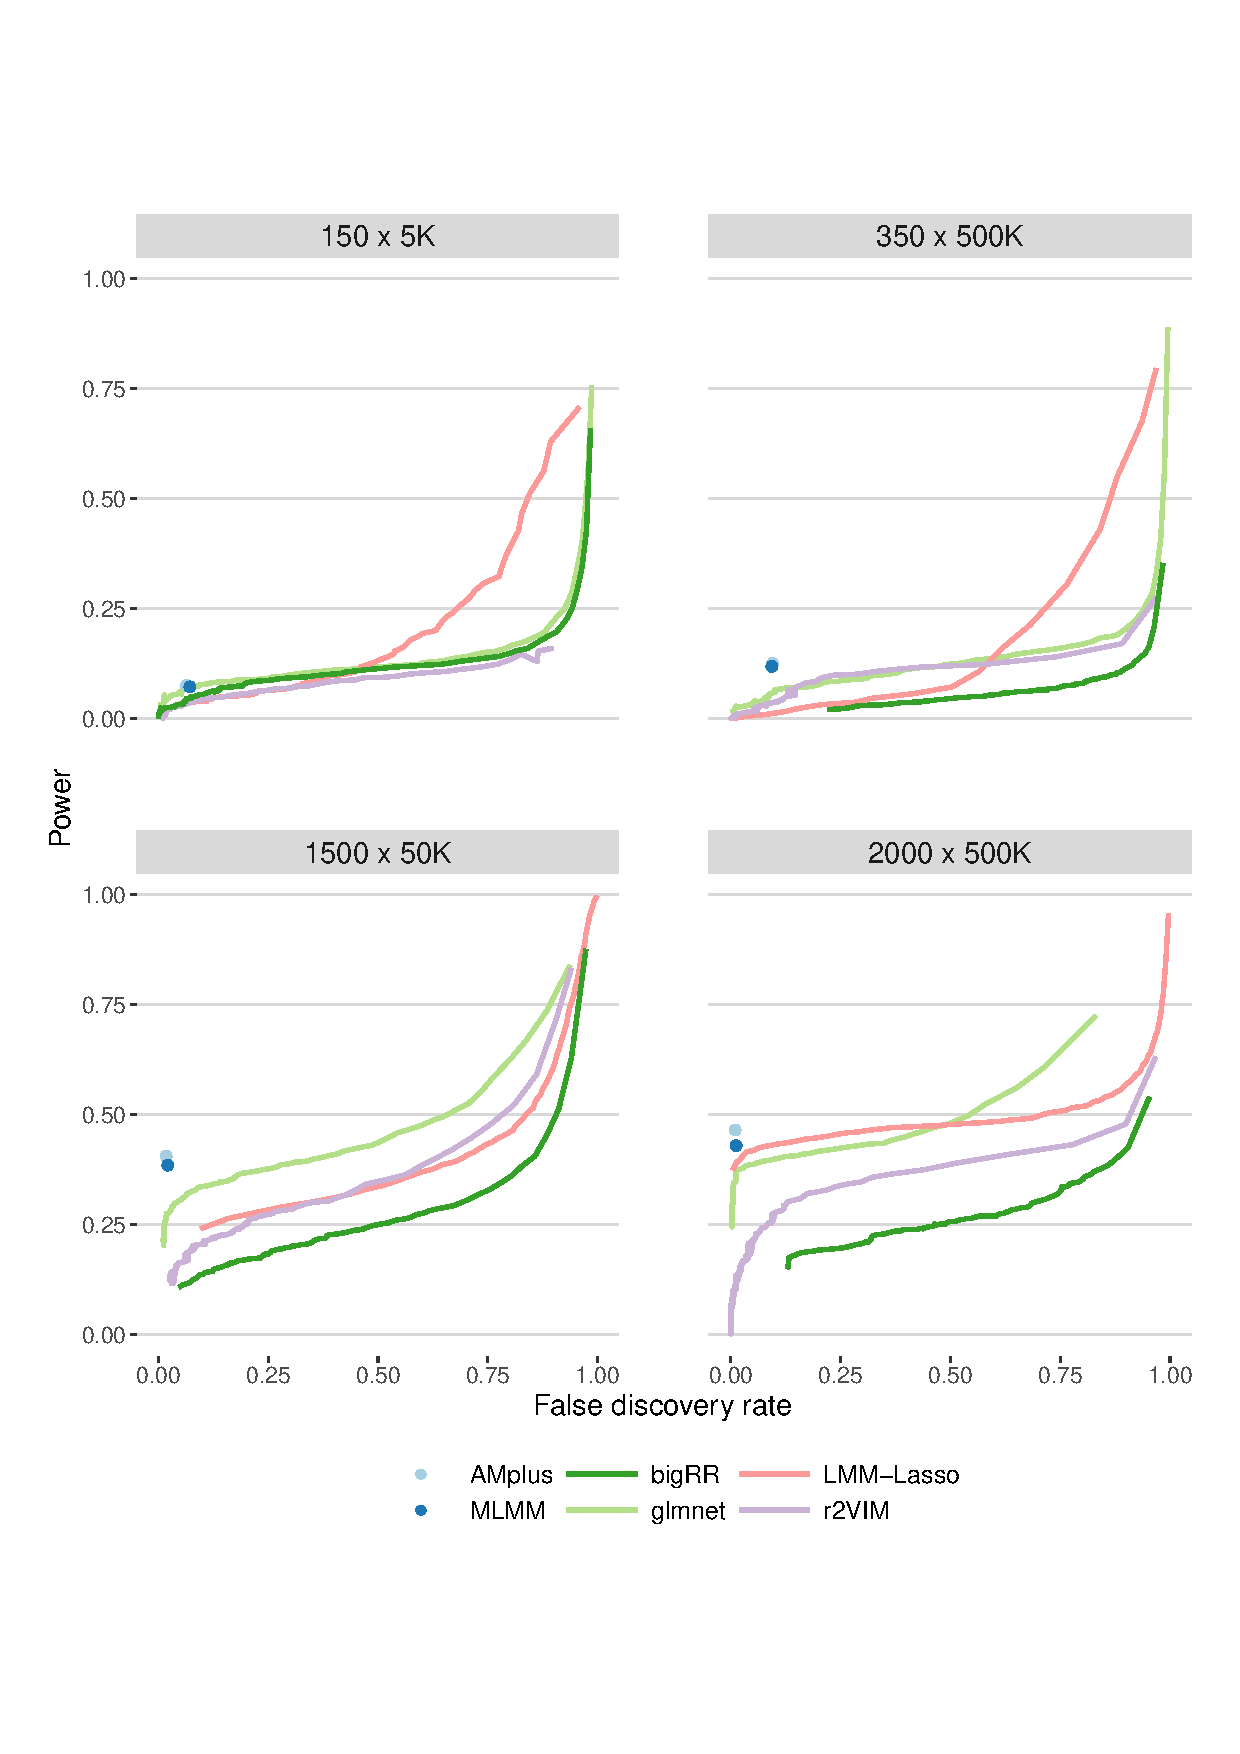
\includegraphics[width=10cm]{powerMultiple}
\end{figure}

\begin{figure}
\label{fig_power_single}
\caption{Power curves for single-locus methods -- Put into sup methods}
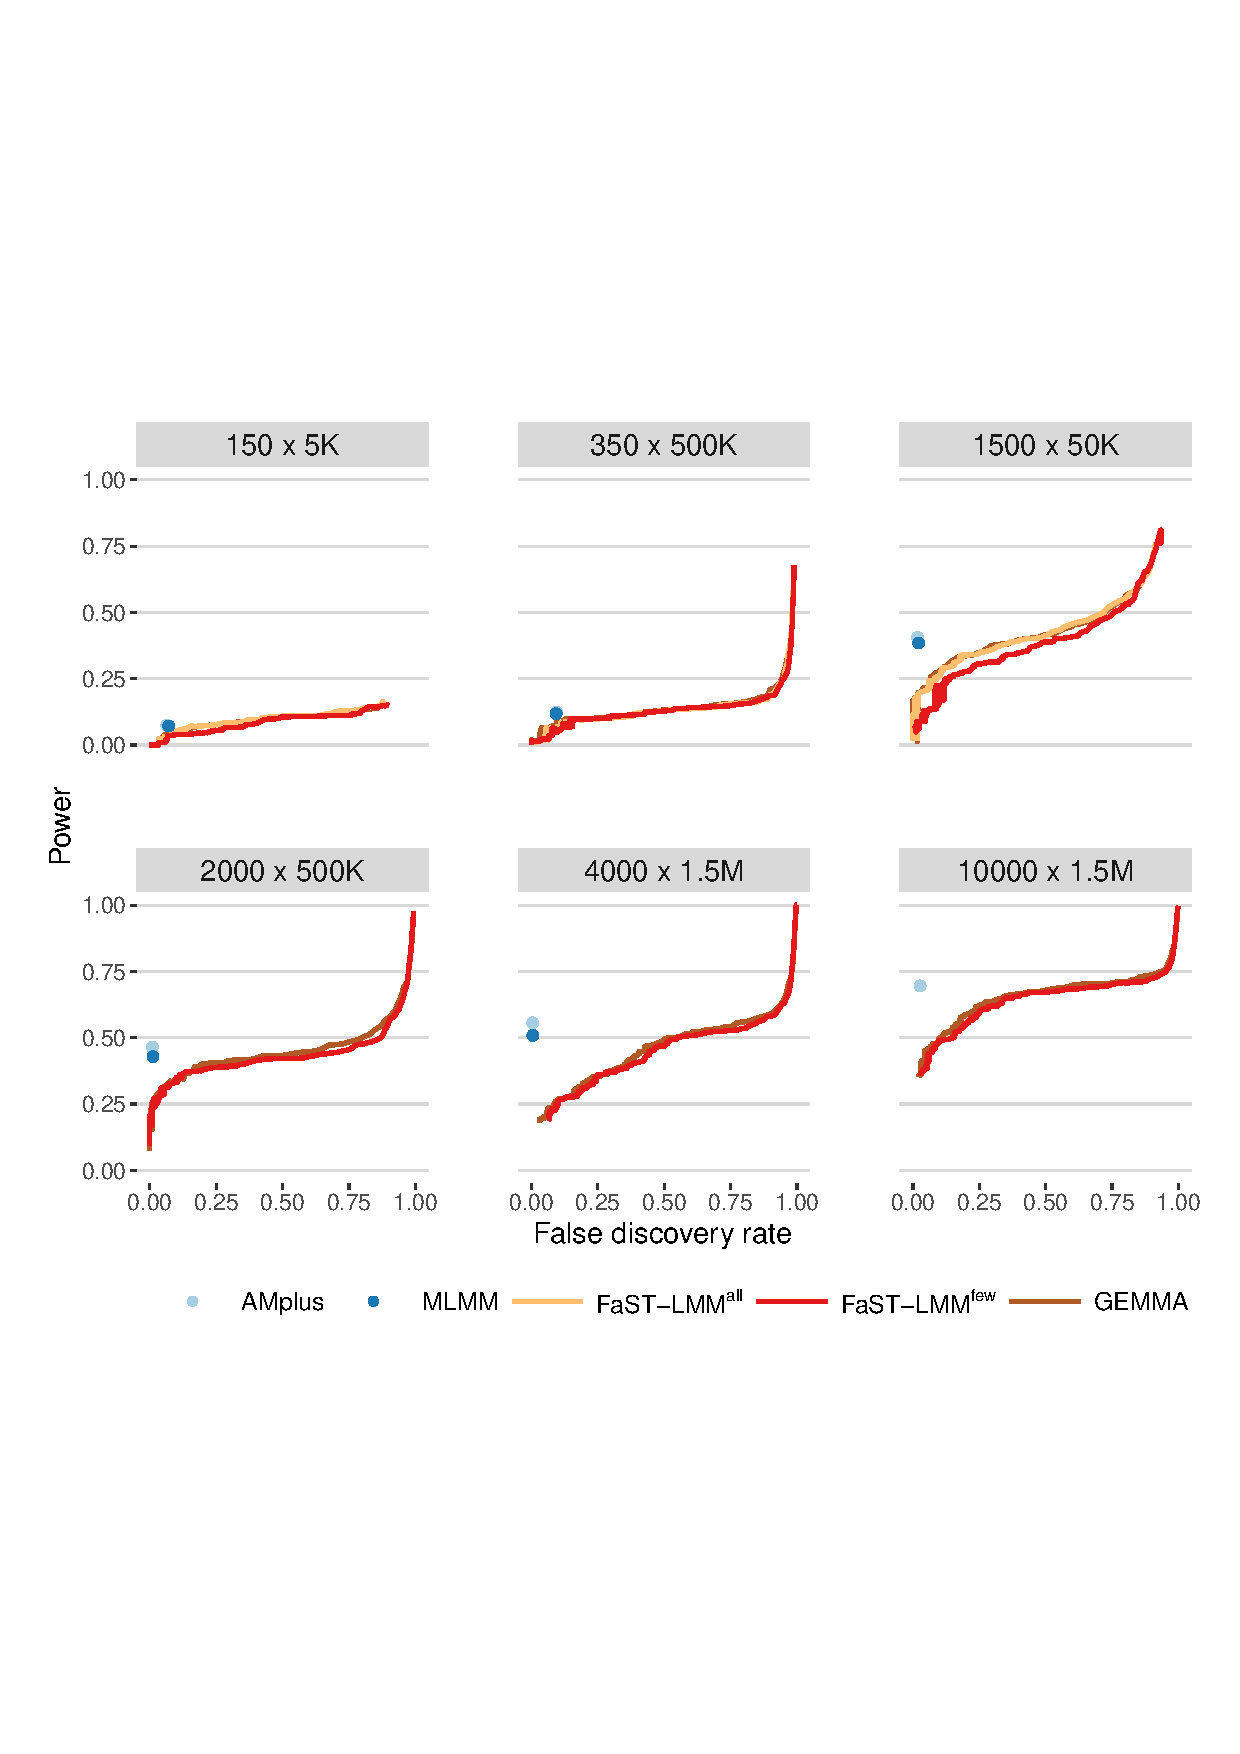
\includegraphics[width=10cm]{powerSingle}
\end{figure}


\begin{figure}
\label{fig_threshold}
\caption{The impact of threshold on FDR }
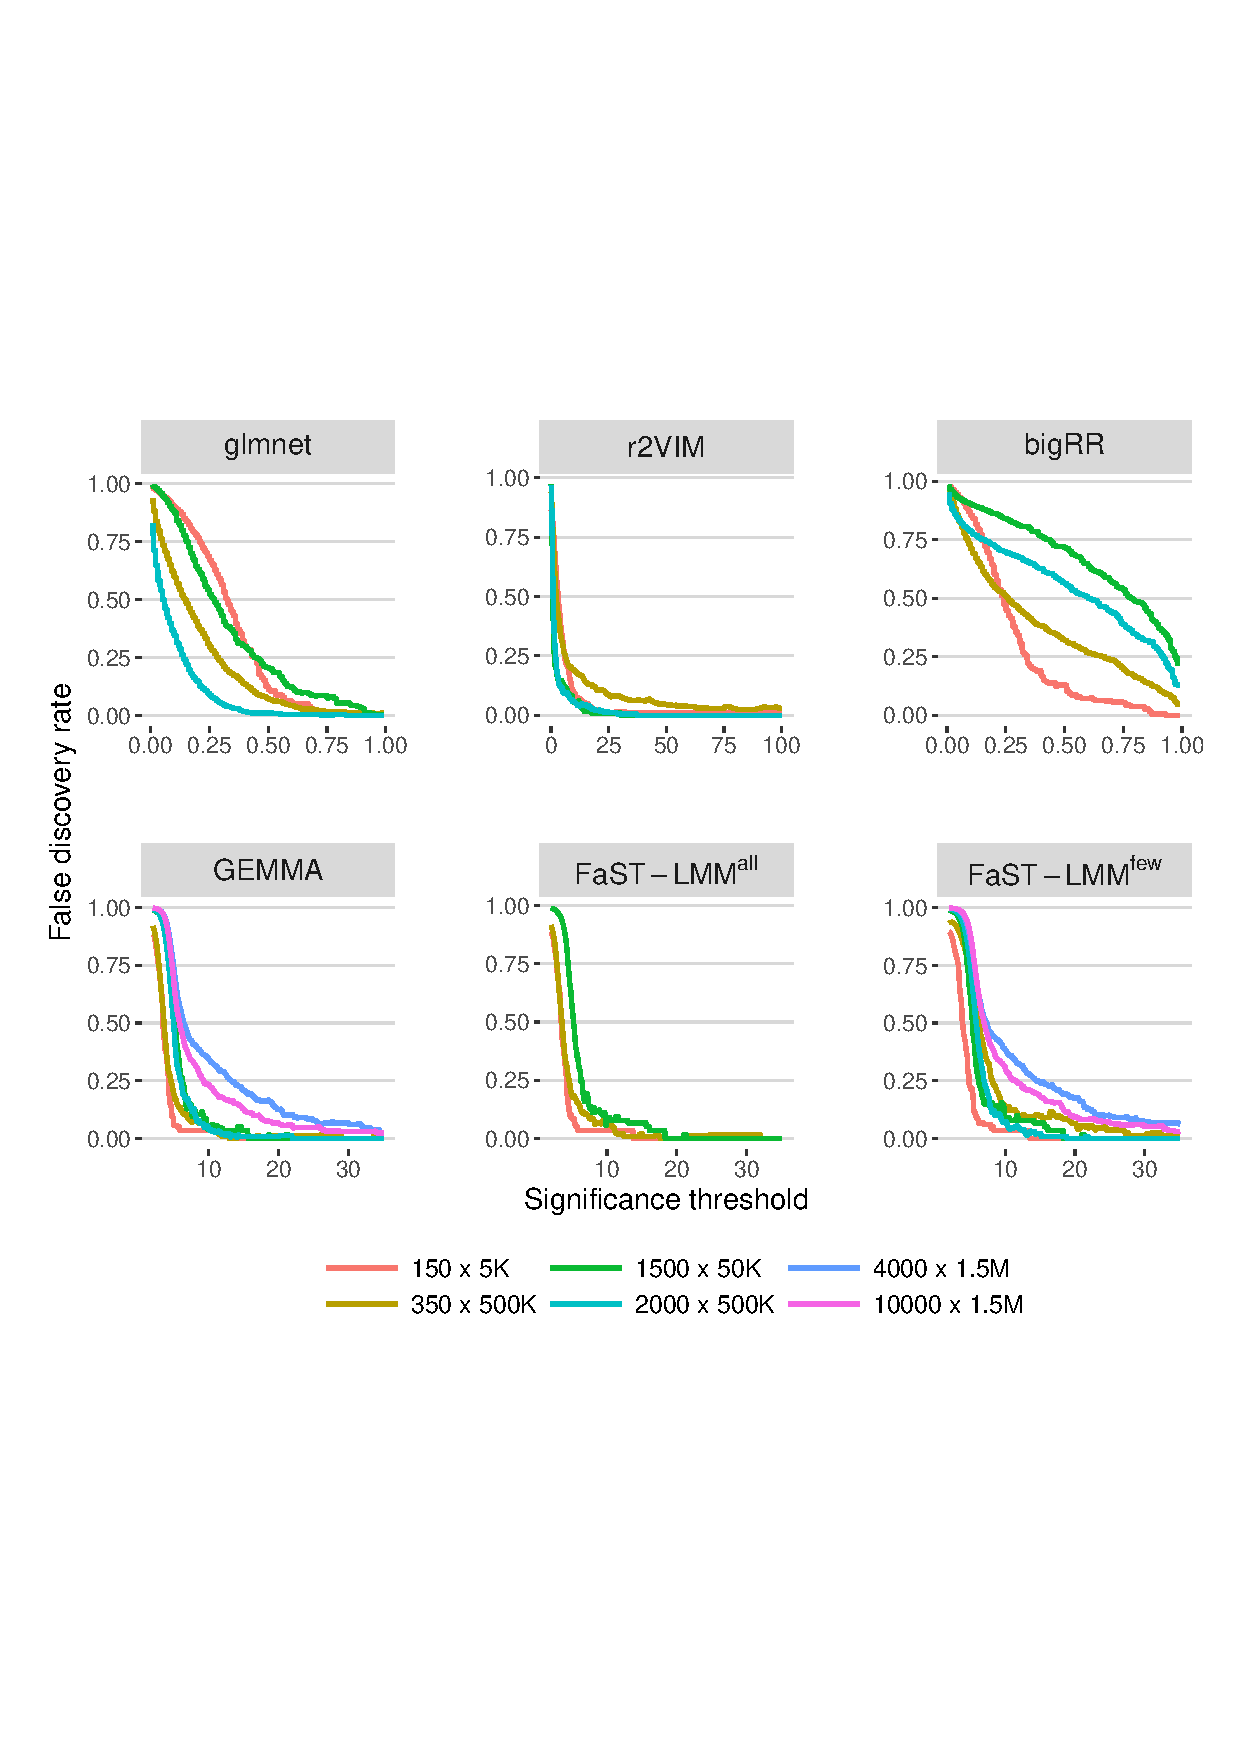
\includegraphics[width=10cm]{threshold}
\end{figure}




\subsection{Mouse Data Analysis}

We were interested in comparing results from Eagle with those from single locus association mapping for a real data set.
 We chose to focus on data from a large outbred mouse study. This study was unusual in that it collected and analysed snp dosages (continuous values from zero to one of expected allele counts)  instead of the more common snp genotypes. Analyses based on dosages rather than discrete genotypes have been shown to have greater power of detection \cite{zheng2011comparison}. By converting the dosages into genotypes and analysing the data with the single locus program FaSt-LMM, we obtained a subset of those findings reported in the original study. We then analysed the data with Eagle. Due to Eagles increased power, we found snp-trait associations not found with the FaST-LMM. However, we were 
 able to confirm the validity of these new findings as they matched what was found in the original study.

For the single locus analysis of the data, we followed the same procedure as xxxx. 
The only exceptions were that we focused on the autosomal snp and it was necessary to 
increase the number of permutations for the controlling of the fdr from 100 to 500.

Eagle was run in two ways; under its default settings ($Eagle^{default}$) and where we specified the regularisation parameter for model selection ($Eagle^{optimal}$ ) Eagle chooses the best model via the extended BIC criteria (ref). The conservativeness of the extended BIC can be adjusted by a single regularisation parameter that ranges from 0 to 1. In the simulation study, this parameter was set to 1, its most conservative and default setting. However, there is also opportunity to set the parameter to a value less than 1. This increases power but also increases the fdr. For each trait, we used permutation to set the regularisation parameter to give a fdr of 5\% .

The genome wide results from the analyses of the mouse data are shown in Figure X. The mouse study took
measurements on 200 traits.  However, we focused our analyses on the 43 traits whose snp-trait associations could be
corroborated by prior published evidence. Each plot contains the number of snp-trait associations that were found and in agreement with the original findings. Neither method found snp not identified in the original mouse study.
As we saw in the simulation study, there is a notable difference in the two methods capacity to discover snp-trait associations. $Eagle^{default}$, under its default settings, for x traits found the same number of findings as FaST-LMM and for y traits found more findings. $Eagle^{optimal}$, 
with its regularisation parameter fine tuned to the trait, for x traits found the same number of findings as FaST-LMM and for y traits 
found more findings. Overall, $Eagle^{default}$ and $Eagle^{optimal}$ found xx\% and yy\% more snp-trait associations than a 
single-locus analysis of the mouse data. 



\section{Methods}

\subsection{Outbred Mice Study}
\subsection{Mouse Data}

The mouse data were obtained from a large genome-wide association study which was performed in outbred mice. 
The study is described in detail in \cite{nicod2016genome}. Phenotypic and genotypic data were available on 1,887 adult mice. 
The phenotypic data consisted of measurements from 200 behavioural, tissue based, and physiological traits.  Of these traits, 
43 yielded snp-trait associations that could be corroborated through other independent published work. It was these 
43 traits which were the focus of our real data analyses. Genotypic data were available on 359, 559 (353,697 autosomal) SNPs in the 
form of marker dosages (expected allele counts that range from zero to one). All missing data had been imputed. 
We converted these  dosages into discrete genotypes 
by clustering around 0, 0.5, and 1, corresponding to SNP genotypes AA, AB, and BB, respectively. 


\subsection{Eagle Approach for Multiple-locus Association Mapping}

Eagle is a method for multiple locus association mapping on a genome-wide scale. It is based on linear mixed models. It differs from most other single- and multiple-locus association mapping methods. Eagle treats association mapping as a model selection instead of parameter estimation problem. Consequently,  we do not have to content with multiple testing issues or having to construct significance thresholds. 
The methodological foundation for Eagle comes from a whole-genome linkage analysis method that was developed for mapping 
quantitative trait loci in experimental crosses \cite{verbyla2007analysis} 


Let $S = \{ S_1, S_2, \ldots, S_s\}$ be a set of ordinal numbers where $S_k$ is the $S_k$th ordered snp that was 
selected in the $k$th iteration. For example, if three iterations of our model building procedure 
have been performed and say the 500023rd, 15th, and 420th, 
snp were selected, then $S=\{500023, 15, 420\}$. 
Let $y^{(n \; \times \;1)}$ be a vector containing $n$ quantitative trait measurements. 
Let $M^{(n_g \; \times \; L)} = [m_1 m_2 \ldots m_L]$ be a matrix containing the genotype data which have been collected 
from $L$ loci that span the genome on $n_g$ groups/lines/strains.  Here, $n \geq n_g$ meaning that several trait measurements 
may be taken of the same group/line/strain. 
 It is common for the columns of $M$ to be in map order but this is not a requirement. 
The vector $m_j^{(n_g \; \times \; 1)}$ contains the genotypes for the $j$th snp. 
The genotypes are coded as -1, 0, and 1 corresponding to snp genotypes AA, AB, and BB, respectively. 

The specifics of the Eagle method are as follows. 
Eagle builds the "best" model iteratively, via forward selection. 
Suppose $s$ iterations of our model building process have already been performed. This means $s$ snp-trait 
associations have been identified.  It also means that $s$ separate genomic regions of interest have been found.  
To perform the $s+1$th  iteration, we first fit the current model to the data. 
The (current) model is of the form 
\begin{equation}
\label{eq1}
y = X \tau + Z u_g + e
\end{equation}
where 
$X^{(n \; \times \; p)}$ and $Z^{( n \; \times \; n_g)}$ are known design matrices with $X$ being of full rank and $Z$ 
containing zeros and ones that assign the appropriate genetic effect to each measurement. 
The vector 
$\tau^{(p \; \times \; 1)}$ has $p$ fixed effects parameters including the intercept. The vector 
$u_g^{(n_g \; \times \; 1)}$ contains the 
genetic effects. The vector of residuals is 
$e^{(n \; \times \;1)}$ whose distribution is assumed to follow $N(0, \sigma^2_e I^{(n \; \times \; n)})$. 
So far,  this model differs little from standard linear mixed models for association mapping (refs). 
However, 
it is how we specify $u_g$ that distinguishes our model from others. 

The genetic effects $u_g$ are modelled as 
\begin{equation}
\label{eq2}
u_g = \sum_{k=1}^s  m_{S_k} a_{S_k} + M_{-S} a_{-S}
\end{equation}
where $m_{S_k}^{(n_g \; \times \; 1)}$ is the vector of genotypes for the $S_k$th snp locus which is the $k$th selected snp, 
$a_{S_k}$ is the additive effect of the $S_k$th snp locus, $M_{-S}^{(b \; \times \; L-s)}$ is the matrix of  snp genotypes 
with the data for the selected snp in $S$ removed,  and $a_{-S}^{(L-s \; \times  \; 1)}$ is a random effect whose distribution is 
$a_{-S} \sim N(0, \sigma_a^2 I^{(L-s \; \times \;  L-s)})$. 
The terms in the summation on the left hand side are fixed effects.  The other term is a random effect.  The terms 
in the summation account 
for the additive effects of genes that are in linkage disequilibrium with the selected snp. The other term models 
snp-trait associations along the entire genome, except for those snp that have already been selected. 
This is a simple genetic model but it 
is effective for discovering snp-trait associations. It also reduces the computational cost of our model building procedure. 


Second, we estimate the parameters of (\ref{eq1}) and (\ref{eq2}) via residual maximum likelihood estimation. 

Third, we identify the $(s+1)$th snp that is in strongest association with the trait, based on the maximum score statistic
$t_j^2 = \frac{ \widetilde{a} _j^2}{\textrm{var}(\widetilde{a}_j)}$ where $\widetilde{a}_j$ is the best linear unbiased predictor (BLUP), 
and $\textrm{var}(\widetilde{a}_j)$ is its variance. This statistic is not only appealing intuitively, where we 
identify a snp based on its (random) effect size and accuracy, but is theoretically justified.  It follows from outlier detection 
in linear and linear mixed models (ref). 

Fourth, we determine the importance of the $(s+1)$th selected snp via a model selection strategy. 
We begin by reforming (\ref{eq2}) where $S$ now contains the $s + 1$ selected snp.  We then fit this new model to the data
via maximum likelihood and calculate its extended Bayesian information criteria (ExtBIC) \cite{chen2008extended}.  The ExtBIC is a model selection measure that takes into account the number of unknown parameters and the complexity 
of the model space.  It is especially well suited to the model selection problem in genome-wide association studies \cite{chen2008extended}. If this new model has a larger ExtBIC than the current model, then the $s+1$th selected snp is added to 
the current model and the above process is repeated. If this new model has a smaller ExtBIC than the current model, then the 
model building process is complete. The set of snp in strongest association with the trait is the $s$ snp previously identified. 

\subsubsection{Reducing the dimension of the model}
In practice, estimating the parameters of (\ref{eq2}) can be demanding, computationally. 
The vector $a_{-S}$ has $L-s$ random effects where in modern genome-wide association studies, 
$L$, the number of snp, can be extremely large.  An alternative model is given by 
Verbyla \cite{verbyla2012rwgaim,verbyla2014whole}. 
They show how to reformulate (\ref{eq2}) to be a model with a random effect with only $n$ elements
\begin{equation}
\label{eq3}
u_g = \sum_{k=1}^s  m_{S_k} a_{S_k} + (M_{-S} M_{-S}^T)^{1/2} a^*_{-S}
\end{equation}
where $a^* \sim N(0, \sigma_a^2 I^{(n_g \; \times \;  n_g)})$, and 
$(M_{-S} M_{-S}^T)^{1/2}$ can be calculated via single value decomposition (ref).  
Although it may not be obvious, the two models are equivalent, 
having identical variance structures. Yet, the computational cost of model (\ref{eq3}) compared to 
model (\ref{eq2}) is much less due to the random term having only $n$ effects needing estimating. 

Verbyla \cite{verbyla2012rwgaim,verbyla2014whole} go on to show how to recover $\widetilde{a}$ from estimates from model (3) with 
\begin{equation}
\widetilde{a} = \left [ M_{-S}^T (M_{-S} M_{-S}^T)^{-1/2} \right ] \widetilde{a}^*
\end{equation}
where its variance matrix is
\begin{equation}
\label{eq4}
\textrm{var}(\widetilde{a}) = M_{-S}^T (M_{-S} M_{-S}^T)^{-1/2} \textrm{var}(\widetilde{a}^*) (M_{-S} M_{-S}^T)^{-1/2} M_{-S}
\end{equation}
These values are needed in order to calculate the score statistic $t_j^2$ for identifying the snp in strongest association with the trait. 
Fortunately, when calculating $t_j^2$, only the diagonal elements of the variance matrix are needed which simplifies the  calculation. 
of (\ref{eq4}). 



\subsection{Comparison Methods}

\subsubsection{Multiple locus methods}

We compared the computational and statistical performance of Eagle against five other multiple locus applications for 
association mapping  These were BigRR, LMM-Lasso, glmnet, MLMM  and, r2VIM. 
BigRR, LMM-Lasso, and glmnet  implement different regression-based regularisation methods. Regularisation methods have dominated 
the development of multiple locus approaches.  They give opportunity for the effect of all the snp to be modelled simultaneously. 
By introducing a penalty function that balances bias and variance, regularisation methods can 
handle parameter estimation problems where the number of predictors is far greater than the number of samples.  
MLMM is similar in philosophy to Eagle in that it treats association mapping as a model building problem. Here, a linear mixed 
model is built through a forward-backward selected strategy.  
R2VIM is different to the others in that it implements 
random forests for association mapping. 
Random forests is a machine learning approach that forms an ensemble of decision trees for regression and 
classification. 
These five methods were selected because of their demonstrated value 
for analysing genetic data, they reflect a range of different statistical methodologies for association mapping, and they are available as 
either stand-alone computer programs or as  packages. A summary of how the computer programs/packages differ in their 
features is given in Table X. Each method is now described in a little more detail. 



\textbf{BigRR:} BigRR \cite{shen2013novel}  is an R package that implements generalized ridge regression.
In ridge regression, the coefficients of the predictors are shrunk 
to zero by a constant amount.  In generalized ridge regression, the amount of shrinkage is allowed to vary, giving opportunity for 
a more realistic model to be specified. The model used in BigRR can be formulated as a linear mixed model that is 
$y = X \beta + M u + e$ where $u^{(L \times 1)}$ is a vector of snp effects, and each snp 
effect is normally distributed with its own variance such that $u_l \sim N(0, \sigma^2_l); l=1,2, \ldots, L$. 
The parameters are estimated via a 
algorithm that makes clever use of the Cholesky decomposition of the genomic relationship matrix, 
and the equivalence between the above model and animal models \ref{stranden2009animalmodel}. 
One of the challenges in using BigRR for association mapping is that while it has the capacity to estimate the effect sizes of all the snp simultaneously, 
obtaining their statistical significance is difficult. 
Permutation has been suggested as a way of calculating significance 
empirically \cite{shen2013novel} but we instead opted for stability selection.


\textbf{LMM-Lasso:} LMM-Lasso  \cite{rakitsch2013lasso} is a stand-alone computer program that implements lasso within a linear mixed model 
framework. Unlike in ridge regression, lasso performs parameter estimation and variable selection, simultaneously.   The 
coefficients of "unimportant" predictors are shrunk to exactly zero.
The (full) model is 
$y =  \sum_{l=1}^L m_l \theta_l +   g  + e$ where $g^{(n ; \times 1)}$ is a vector of random polygenic effects such that 
$g \sim N(0, \sigma^2_g K)$, and $K^{(n ; \times \; n)}$ is a realised relationship matrix reconstructed from the snp information. 
It is challenging, computationally,  to apply lasso directly to the full model for parameter estimation. Instead, a two step procedure 
is adopted. In the first step, the above model without any snp effects is fitted. In the second step, 
the unknown variance components in the full model are replaced by their estimates 
that were calculated in the first step. Lasso is then applied to this simpler model making lasso more tractable, computationally. 
As with BigRR,  the statistical significance of the snp effects are not calculated. We use stability selection to obtain the 
significance empirically. 

\textbf{Glmnet:} Glmnet  \cite{Friedman2010glmnet}, unlike BigRR and LMM-Lasso, was not purpose built for 
association mapping.  It is a general R package for 
regression analysis. We have included it in our list of applications for comparison with Eagle because the 
regularization method, elastic net, upon which the package is based has been found to be superior to ridge regression and 
lasso (ref needed???).  Elastic net uses a penalty function that is a mixture of 
$\ell_1$-norm (lasso) and $\ell_2$-norm (ridge regression) penalties  \cite{zou2005regularization}. 
This allows elastic net to avoid the limitations of lasso 
while still being able to perform shrinkage and variable selection, simultaneously. 
Glmnet can handle a range of different models. For the analyses performed in this paper, the model is 
$y = X \beta + \sum_{l=1}^L m_l \theta_l + e$ where $\theta_l; l=(1,2, \ldots, L)$ is the coefficient for the $l$th snp. 
We used stability selection to obtain the significance of the coefficients (snp effects). 


\textbf{MLMM:} Of the multiple-locus applications considered in this paper, 
MLMM \cite{segura2012efficient} bares the greatest similarity to Eagle algorithmically.  MLMM, like Eagle, performs 
association mapping by building the "best" linear mixed model.  The model used for analysis 
is the same as (\ref{eq1}) except that the genetic effect is 
\begin{equation}
\label{eqmlmm}
u_g = \sum_{k=1}^s  m_{S_k} a_{S_k} + g
\end{equation}
where 
$g^{(n ; \times 1)}$ is a vector of random polygenic effects with distribution 
$g \sim N(0, \sigma^2_g K)$. The model is built iteratively, via forward-backward variable selection.  In Eagle, at each iteration, 
the snp in strongest association with the trait is found by calculating the score statistic $t_j^2$.  In MLMM, at each iteration, 
a separate linear mixed model analysis is performed for each snp not already selected. The snp yielding the most 
significant result (lowest p-value) is selected for inclusion in the fixed effects part of (\ref{eqmlmm}).  
Two selection 
criteria are available for the model building process: 
the EBIC and the multiple-Bonferroni criterion. We used only the EBIC. 



\textbf{r2VIM:} R2VIM is an R package specifically designed for association mapping \cite{szymczak2016r2vim}. 
It implements random forests and a new way of measuring the importance of a snp.  In random forests, the worth of a predictor is measured, empirically, by calculating its importance score. It is from these importance scores that snp can be ordered in terms of their strength of association with a trait. The challenge though is in knowing what proportion of the 
highest ordered snp are in true association. R2VIM addresses this by calculating a relative importance score for a snp. Briefly,
$m$ random forest analyses of the data are performed. Each analysis is reliant upon a different random number seed. 
From an analysis, a relative importance score for a snp is obtained by taking the ratio of its importance score to the absolute 
minimum of the importance scores across all the snp.  Those 
snp with high relative scores across all $m$ analyses are deemed to be of interest \cite{szymczak2016r2vim}.
Applying r2VIM to the analysis of GWAS data is not without its challenges.  First, it is not possible to force every 
decision tree to have important (fixed) effects without a change to the internal workings of the r2VIM package. 
So we adopted a two step 
strategy. In the first step, the fixed effects are regressed on to the trait and the residuals recorded.  In the second step, 
r2VIM is employed were the trait data are the residuals obtained from the first step. This is not ideal (ref to problems with two
step approaches).  Second, there is no relationship between relative importance scores and significance levels. Consequently, 
setting an appropriate genome-wide threshold is problematic. We avoid this problem by focusing, in the simulation study, 
only on the relationship between threshold level and its false discovery rate and power. 

\subsubsection{Single locus methods}

We were also interested in comparing Eagle to single locus methods to measure the difference in run times and statistical power. Even by limiting our focus to LMM-based methods, there were a number of efficient applications to choose from. 
We decided on GEMMA \cite{zhou2012genome} and FaST-LMM \cite{lippert2011fast}. These two applications have the same computational complexity \cite{zhou2012genome}, produce exact instead of approximate results, and are highly efficient computationally. They were developed at the same time, independently, but are very similar theoretically. Both perform a single spectral decomposition of the relationship matrix $K$. Both use the eigenvector matrix to rotate the data. Both reformulate the log likelihood and 
restricted/residual maximum-likelihood (REML) 
log likelihood into a sum of $n$ terms that are easier to compute. The difference lies in their estimation procedure. FaST-LMM implement's the Brent's algorithm to optimise $\delta$. GEMMA instead implement's the Newton-Raphson algorithm. Newton-Raphson is more complicated in that it also requires the first and second derivatives of a function to be calculated. However, it is superior in terms of its convergence properties to the Brent algorithm.  Both applications are stand-alone computer programs, popular, and in common use.


\section{Stability Selection}
When using BigRR, LMM-Lasso, and glmnet, the results are affected by the amount of regularization ($\lambda$). 
BigRR has an approximate way of setting each snp's separate regularization parameter (ref). However, the optimal value of 
$\lambda$ must be found when using LMM-Lasso and glmnet. Also, 
all three applications yield the effect sizes of the snp across the entire genome but not their statistical significance. To address 
these issues, we made use of stability selection \cite{meinshausen2010stability}. 
Stability selection is a resampling strategy.  With stability selection, we were able to avoid having to optimise $\lambda$ while 
still being able to calculate, empirically, the statistical significance of the snp effects.

We performed stability selection as follows. For LMM-Lasso and glmnet, we performed a preliminary analysis to find an 
appropriate value for the regularization parameter.  We adjusted $\lambda$ so that they yielded 
between 10 to 30 snp with non-zero effects. Fortunately, with stability selection, the setting of $\lambda$ does not have to be exact 
but limiting LMM-Lasso and glmnet to only 10 to 30 non-zero effect sizes was straightforward. We then repeatedly subsampled, 
without replacement, the data. As recommended \cite{meinshausen2010stability}, we draw 100 subsamples of size $n/2$. We 
analysed the subsample, with $\lambda$ fixed for LMM-Lasso and glmnet.  To calculate, empirically,  the statistical significance of each 
snp across the genome, we counted the number of times a snp had a non-zero effect size over all the replicates to the total 
number of replicates (which was 100). 


For BigRR, we modified our stability selection procedure slightly. 
There was no need to find an appropriate value for the regularization 
parameters as the BigRR package has an internal procedure for their 
calculation. We draw subsamples as above and analyzed the data with BigRR. However, within an analysis, we ordered 
the snp according to the absolute size of their snp effects and recorded the top 20 snp. We then measured the significance 
of the snp across the entire genome as above. 


\cite{meinshausen2010stability}


\section{Simulation Study}

To explore the computational and statistical performance of Eagle, we conducted a large simulation data.  Genome-wide data 
were generated under five different scenarios. These scenarios were data where the sample size was X and the number of snp Y (X x Y) ,

We generated data under five different scenarios. 


We generated 
replicates via data perturbation (ref: Zhao et al. 2007).


These are a GWAS of size 150 individuals and 5000 snp (150 X 5K), 350 individuals and 400000 snp (350 X 400K),  1500 individuals and 
50000 snp (1500 x 50K), 2000 individuals and 500000 snp (2000 x 500K), 4000 individuals and 
1500000 snp (4000 x 1.5M), and 10000 individuals and 1500000 snp (10000 x 1.5M).  
We chose these scenarios to reflect some of the different sized GWAS being performed in animals, plants, and humans. 
For each scenario, we generated 100 replicates of data. A single replicate consists of snp genotype data and quantitative trait data. 
We obtained the snp data from the publicly available 1000 genome project (phase 3). The quantitative trait data we generated from the 
snp data by selecting a set of snp loci, assigning allelic effects to these snp, and aggregating these effects for each individual along with 
random error. The number of snp selected per replicate follows a Poisson distribution with mean 30.
 The quantitative trait was generated to have a heritability of 50\%.
Analyses were performed on a high end desktop computer. It had dual 8-core Xeon processors, three Kepler Tesla GPUs, and 128 Giggabytes of RAM. All implementations except, GEMMA, made use of distributed computing, either explicitly or implicitly through multi-threaded BLAS/LAPACK libraries. 




Replicates are generated with data perturbation (Zhao et al. 2007). Data perturbation makes use of the phenotypic and genotypic data observed in a real study to create a simu- lated (quantitative) trait. It affords us the opportunity to generate replicates whose analysis more closely mirrors the complexities of analyzing real data. For computational expediency, our simulation study is based on data observed from the Biloela site in 2006. In generating trait data for a replicate, we assume a broad based heritability of 0.6, there is a single major QTL, the polygenic component consists of 30 polygenes where the effect of a polygene is formed from an unmapped SNP which was chosen randomly, and the variance structure of the simulated trait closely follows that of the loaf volume trait. The marker data consists of those genotypes collected in the association study from the 3129 SNP across the 21 homologous chromosomes. Each replicate has the same marker data. It is the simulated trait data that varies across replicates.
Our simulation study consists of three parts. First, we conduct a null study to investigate whether our Monte Carlo sampling approach controls correctly the genome- wide type I error rate. We also evaluate the impact of assuming a block diagonal structure for V. We do this by
also calculating the genome-wide type I error rates when the variance matrix for the joint distribution of the test sta- tistic is formed from loci pairings across the entire genome. Ten thousand replicates are generated where the QTL has no effect. Results are reported for QK-based association mapping implemented as a single-stage and weighted two- stage analysis.
Second, a power study is performed to investigate if there is a difference in performance between implementing QK-based association mapping as a single-stage analysis versus a two-stage analysis. Data are generated under QTL of different sizes and with varying percentages of missing marker data (1.1, 5, 9, 11 %). Missing marker genotypes are imputed for a marker locus by coding its SNP geno- types as ?1 and 1, normalizing its marker data, and replac- ing missing genotypes with zero values. One thousand replicates are generated for each of the four different per- centages of missing marker data and each differently sized QTL. A genome-wide signi cance level of 5 % is assumed.
Third, a study to evaluate our heuristic procedure for choosing between single-stage and two-stage analysis is performed. Data are generated under a QTL of no, mod- erate, and large effect. One thousand replicates are gen- erated for each differently sized QTL. The performance of our heuristic procedure is measured by calculating the proportion of replicates for which the analysis type is inferred correctly. To determine if a single-stage analy- sis is truly needed, it is necessary to analyze fully the genome-wide data via single-stage and weighted two-stage analysis. Then, for each marker locus j, perform the test
| ? log padj ? log qadj| > | ? log padj ? 1.3|, where we have jjj
assumed a genome-wide signi cance level of 5 %. If true, an incorrect  nding occurs if our heuristic procedure deter- mines that it is valid to implement two-stage analysis.
\section{Implementation}

\section{New section written on iPhone added 5 Feb 2018}
\section{Simulation Study}
We conduct a large simulation study to examine the performance characteristics of Eagle. Genome-wide data are generated under five different scenarios. These are a gwas of size 150 individuals and 5000 snp (150 x 5K), 350 individuals and 400000 snp (350 x 400k), 1500 individuals and 50000 snp (1500 x 50k), 200 individuals and ..... We chose these five scenarios to reflect some of the different sized studies being run in animals, plants, and humans. For each scenario, 100 replicates are generated.

To generate a replacate, we used data perturbation (ref). Data perturbation makes use of real genotype data from which a (quantitative) trait is created.
With data perturbation, we are able to preserve some of the challenges of analysing real data while still having trait data whose genetic architecture is known.

The genotype data comes from the 1000 genome project, version 3 (ref). The original data contains X individuals with XX XX snp. From these data, according to the specifications of the scenario, the individuals and the snp loci are identified at random. What about polymorphic affect numbers? Chech).

To generate the quantitative trait data, first the number of snp that are to be in complete with an underlying qtl (x) is drawn from a poison distribution with mean equal to 30. Second, x snp loci are select randomly from a scenario?s set of genotype data. Third, the snp values are summed across the selected loci for each individual to generate a vector of n genetic values. Here, each snp is having, roughly, the same effect on the trait, remembering that the maf of a snp also impacts a snps influence on a trait. Fourth, n deviates are drawn from a $N(0,sigma^2_e)$ where $\sigma_e^2$ has been set to yield a trait with a heritability of 0.6. (Put in formula). Fifth, the quantitative trait data is generate as $y = g + e$. In this way, the same genotype data are used, within a scenario, for all replicates. Only the quantitative trait data varies across replicates.




\section{Implementation}

Eagle has been implemented as an R package of the same name. However, much of the calculation is performed through c++ functions for improved performance. Eagle has been specially designed to harness the multithreaded math libraries blast and lapack but it will run on a single processor computer. It can also deal with data larger than the memory capacity of a computer. Eagle can be run as a standard R package or via the web based GUI. The GUI relinquishes the need to know R to use Eagle.


Eagle can be downloaded from CRAN and installed in the usual way. A containerised version of Eagle is also available. It is built with singularity (ref). This container already has Eagle installed on a multi-threaded version of R. The container is downloaded as a single file from ccxx


A quick start guide, how to videos, installation instructions, and answers to frequently asked questions are available at the Eagle website (http://...)



$------$




We compared the performance of Eagle against seven other association mapping applications. 
Five of these applications, BigRR, glmnet, FaST-LASSO, MMLM, r2VIM implement methods that have been applied to the multiple locus analysis of data from genome-wide association studies. 
The other two applications, GEMMA, and FaST-LMM implement single-locus association mapping methods. 
The packages 
differ in their features (summarized in Table X).  The packages also differ in their underlying methods (summarized below). 

\subsubsection{Multiple locus methods}

\textbf{BigRR:}  In the BigRR package,  generalised ridge regression is implemented  for
the analysis of genetic data \cite{shen2013novel}.  Generalised ridge regression 
 is a regularisation method in that it produces regression solutions 
that have higher bias than ordinary least squares but reduced variance for improved prediction accuracy. The underlying 
model is  $y = X \beta + M u + e$ where $u^{(L \times 1)}$ is a vector of genetic effects, and each genetic 
effect is normally distributed with its own variance such that $u_l \sim N(0, \sigma^2_l); l=1,2, \ldots, L$.  The 
amount of shrinkage is allowed to vary across the genetic (snp) effects. This differs to 
standard ridge regression where the shrinkage is constant. 
Generalised ridge regression is apt at estimating the effect sizes of snp on a genome-wide scale but  obtaining their 
statistical significance analytically is difficult. Shen \cite{shen2013novel} suggested permutation as a way of calculating significance 
empirically. We instead opted for stability selection (see below of details). 



\textbf{glmnet:}  Glmnet is a general purpose R package for regression analysis  \cite{Friedman2010glmnet}. 
The model used for analysis is 
$y = X \beta + \sum_{l=1}^L m_l \theta_l + e$ where $\theta_l; l=(1,2, \ldots, L)$ is the coefficient for the $l$th snp. 
All snp effects are modelled, simultaneously. 
Glmnet implements elastic net for the estimation of the parameters. Elastic net is a regularisation method where the 
penalty function is a mixture of 
$\ell_1$-norm (lasso) and $\ell_2$-norm (ridge regression) penalties  \cite{zou2005regularization}. 
This allows elastic net to avoid the limitations of lasso 
while still being able to perform shrinkage and variable selection, simultaneously \cite{zou2005regularization}. 
Glmnet was not specifically built for association mapping. 
However, it is included in our list of comparison applications due to its solid performance for genomic prediction 
\cite{heslot2012genomic,ogutu2012genomic}.
The glmnet package 
implements a modification of the LARS algorithm \cite{efron2004least} for finding the optimal regularisation (solution) path. 
From exploratory analyses of the simulated data, we found this algorithm yielded a high proportion of false positives. 
We instead fixed the shrinkage parameter to a suitable value 
and employed stability selection to estimate the significance of the snp coefficients, empirically (see below).  



\textbf{LMM-Lasso:} LMM-Lasso is a stand-alone computer program for association mapping within a linear 
mixed model framework \cite{rakitsch2013lasso}. The (full) linear mixed model used for analysis is 
$y =  \sum_{l=1}^L m_l \theta_l +   g  + e$ where $g^{(n ; \times 1)}$ is a vector of random polygenic effects such that 
$g \sim N(0, \sigma^2_g K)$, and $K^{(n ; \times \; n)}$ is a realised relationship matrix reconstructed from the snp information. 
All snp effects are modelled, simultaneously. However, a limitation of this model is its inability to accommodate 
additional fixed effects (there is no $X \beta$ term). 
The parameters are estimated via lasso \cite{Tibshirani1996lasso}. Lasso is a regularisation method with the capacity to perform parameter estimation and variable selection, simultaneously.  
Lasso is computationally intensive, especially when applied to linear mixed models. To avoid this problem, a two-step 
estimation procedure is adopted.  In the first step, the above model but without any snp effects is fitted via 
maximum likelihood. In the second step, the unknown variance components in the full model are replaced by their estimates that were calculated in the first step.  This turns the full model from a linear mixed model into a simpler linear model. Here, lasso is far more tractable, computationally.  To assess the significance of the snp coefficients, as suggested \cite{rakitsch2013lasso}, we implemented stability selection (see below). 


\textbf{MLMM:}  Of the multiple-locus applications considered in this paper, 
MLMM bares the greatest similarity to Eagle algorithmically.  MLMM, like Eagle, performs 
association mapping by building the "best" linear mixed model.  The model used for analysis 
is the same as (\ref{eq1}) except that the genetic effect is 
\begin{equation}
\label{eqmlmm}
u_g = \sum_{k=1}^s  m_{S_k} a_{S_k} + g
\end{equation}
where 
$g^{(n ; \times 1)}$ is a vector of random polygenic effects with distribution 
$g \sim N(0, \sigma^2_g K)$. The model is built iteratively, via forward-backward variable selection.  In Eagle, at each iteration, 
the snp in strongest association with the trait is found by calculating the score statistic $t_j^2$.  In MLMM, at each iteration, 
a separate linear mixed model analysis is performed for each snp not already selected. The snp yielding the most 
significant result (lowest p-value) is selected for inclusion in the fixed effects part of (\ref{eqmlmm}).  
Two selection 
criteria are available for the model building process: 
the EBIC and the multiple-Bonferroni criterion. We used only the EBIC. 

\textbf{r2VIM:} R2RIM is an R package specifically designed for association mapping \cite{szymczak2016r2vim}. 
It implements random forests and a new way of measuring the importance of a snp.  In random forests, the worth of a predictor is measured, empirically, by calculating its importance score. It is from these importance scores that snp can be ordered in terms of their strength of association with a trait. The challenge though is in knowing what proportion of the 
highest ordered snp are in true association. R2VIM addresses this by calculating a relative importance score for a snp. Briefly,
$m$ random forest analyses of the data are performed. Each analysis is reliant upon a different random number seed. 
From an analysis, a relative importance score for a snp is obtained by taking the ratio of its importance score to the absolute 
minimum of the importance scores across all the snp.  Those 
snp with high relative scores across all $m$ analyses are deemed to be of interest \cite{szymczak2016r2vim}.

  
  


\subsubsection{Single locus methods}

\textbf{FaST-LMM:}  FaST-LMM is a highly efficient stand along computer program for association 
mapping \cite{lippert2011fast}. It is based on a standard single-locus model 
\cite{yu2006unified,zhao2007arabidopsis}. Its computational efficiencies come through factorising $K$ with spectral decomposition so that $K=U (S + \delta I) U^T$ where $U$ contains the eigenvectors and $\delta$ is the ratio of the genetic variance to the residual variance. 
By rotating the data with $U$, the log likelihood of the linear mixed model can be expressed as the log likelihood for a simple 
linear model.  This greatly reduces the computational cost of performing lmm-based  association mapping. With FaST-LMM, 
analyses scale linearly with sample size $n$, both in terms of run-time and memory usage.

\textbf{GEMMA:}  to be done. 

\section{Discussion}













%%\bibliographystyle{naturemag}
\bibliography{biblibrary}


\begin{addendum}
 \item Put acknowledgements here.
 \item[Competing Interests] The authors declare that they have no
competing financial interests.
 \item[Correspondence] Correspondence and requests for materials
should be addressed to A.B.C.~(email: myaddress@nowhere.edu).
\end{addendum}



\end{document}
